\section{Data Collection} % < 1.5 Pages

% Outlines:
% - What gestures we want to recognise, based on papers from lit review (maybe own small section?)
% - Taking a data driven approach, what data will we collect

% Distinguishing Between Head and Phone Movement (Methodology)
%   Redefine goals of the system/research objectives
%   Rough outline of the technology we aim to use?
%   Outline data we need

This section details the process undertaken to develop the system which can meet the goal (outlined in \autoref{sec:intro}): distinguishing between head and phone based gestures on a smartphone.

% \subsection{Data Collection Study} % < 1.5 Pages
% outline
% - Taking data driven approach (intro to section)
% - The data we'll be collecting

In order to develop the aforementioned system we opted to take a data-driven approach.
%  The benefit of taking a data-driven approach is that we can leverage Machine Learning, and train the system with exemplar data, rather than needing to manually determine the features and derive the algorithm needed to accomplish our goal.

For a data-driven approach to work we need to first determine what data we need to collect in order to train our system. We have identified the following types of data:
\begin{description}
    \item[Images From The Front Facing Camera]\nl 
    Though a depth camera would likely be more reliable and accurate in extracting the shape/pose of the user's face, it does require hardware that is not yet standard on all smartphones. To enable our system to be run on as many smartphones as possible we will be opting to detect and track the user's head via the front-facing camera, for which we found many techniques from which to extract the user's head movement~\cite{varona2008hands, lopez2012head, viola2004robust, kim2017real, neto2012real, francone2011using, yan2021fast}.
    \item[Smartphone IMU Data]\nl 
        To understand whether the smartphone's PoV is changing we need to know how it is moving. 
        As noted in our review of surrounding literature, the most feasible means to do this is with the IMU present in modern smartphones~\cite{mantyla2000hand, kratz2013combining, neelasagar2015real, garcia2014contextualized}, which will allow us to track the phone's linear and angular acceleration.
    % \item[Head Acceleration Data]\nl 
    %     If we can determine the movement of the smartphone via acceleration data, it is reasonable to see if we can also do the same with the user's head.
    \item[Ground-Truth Data]\nl 
        In order to accurately train a model that can achieve our goal, we will need some Ground-Truth data. This will include the gesture the data is associated with, so that the system can classify gestures. It will also be helpful to capture the actual head and phone poses/motion during given gestures such that we can aim to train a model that can predict the movement of the head and phone.
\end{description}

% - The tools and apparatus we'll be using
% - The data collection app (how it works, issues, output format)
% - Gestures we chose to collect (based on lit review systems, (only subset of pointing, only looking at 8 points around the screen, rather than anywhere))
\subsection{Apparatus and Techniques}

\subsubsection{Pixel 4a}\nl
To collect images and IMU data we opted to use a Pixel 4a smartphone.
The operating system is Android 12, and the phone's dimensions are 144mm x 69mm x 8, with a screen size of 5.6 inches.
This was chosen as it we believe it to be fairly representative of modern smartphones (at least for the android market share), with reasonable dimensions that should not be too difficult to hold for our participants, a front-facing camera capable taking up to 1080p resolution images, an IMU, and a sufficiently powerful processor such that we should not need to worry about an application that can record photos and capture IMU data stuttering and missing data.

\subsubsection{Data Collection Application}\nl
\begin{figure*}
    \centering
    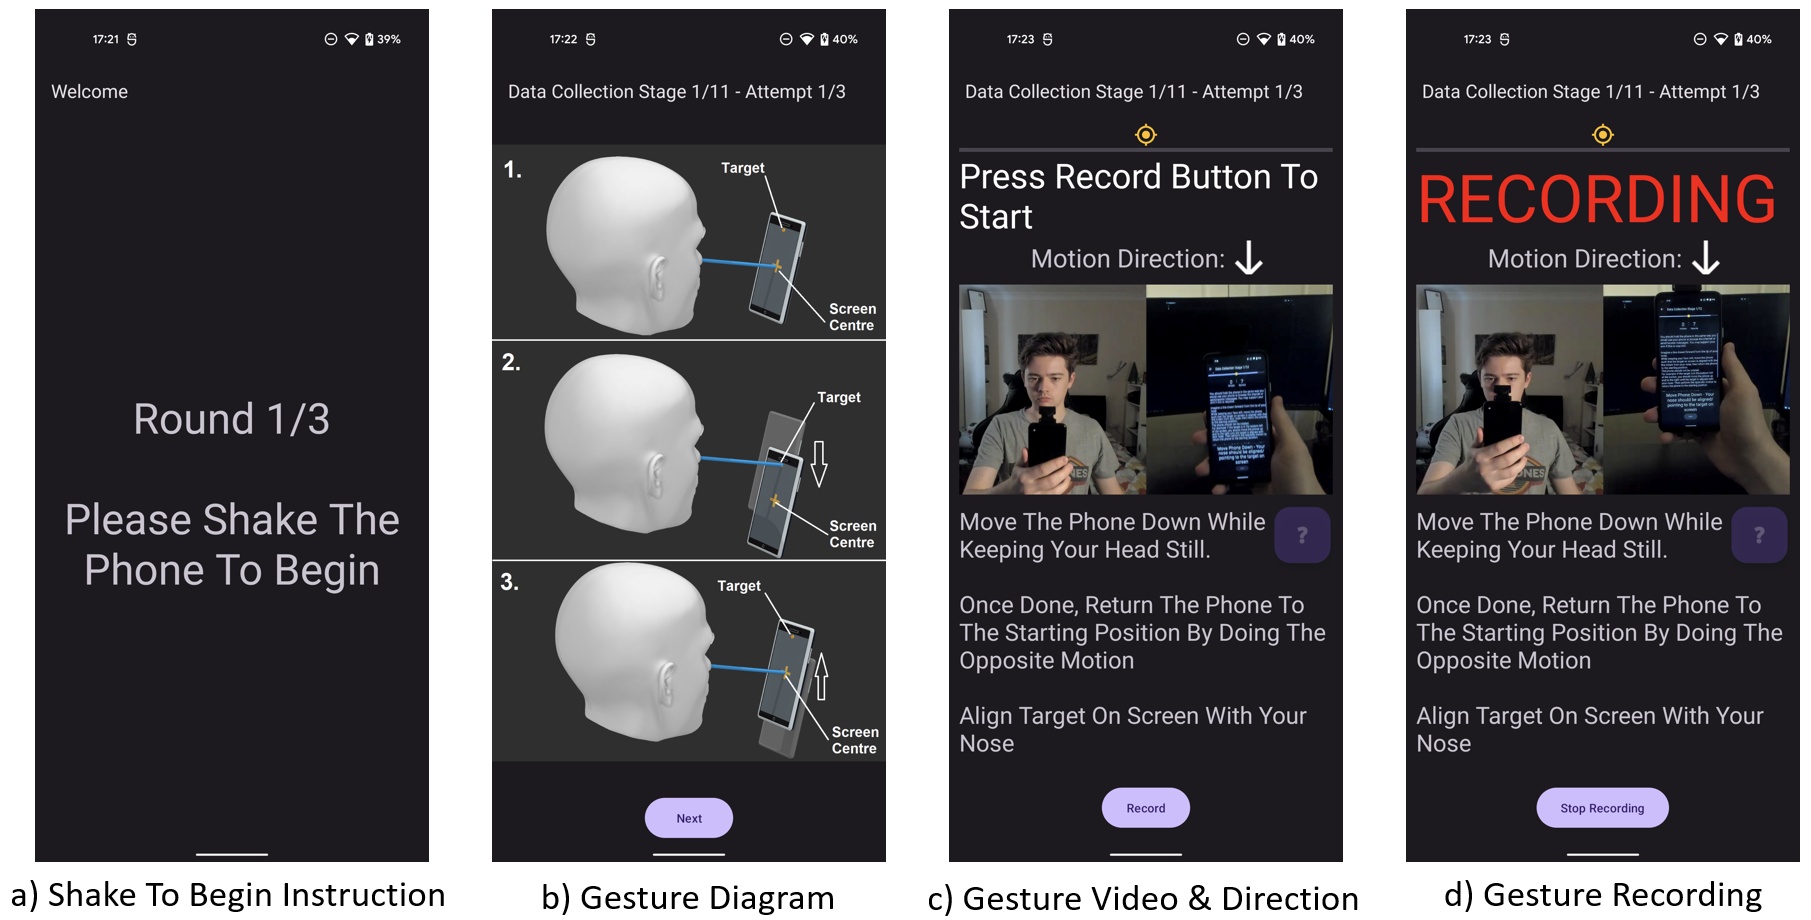
\includegraphics[width=\textwidth]{figures/DataCollectionApp.png}
    \caption{\label{fig:data_collection_app} Various stages of the data collection app UI}
    \Description{Figure showing 4 stills taken from our data collection app. A: Instructions asking participant to shake the phone to start. B: Diagram showing how to perform upcomming gesture. C: Video showing how to perform current gesture, with POV from phone camera and user POV, along with additional symbolic and textual direction cues. D: Application informing participant that data is being recorded.}
\end{figure*}
% Discuss how the application will collect data (images and need to save as raw yuv bytes, IMU with $50Hz$ sample rate saved to csv)
% How data will be organised
% How app will provide instructions
% Shake detection for synchronising with ground-truth data
Since the Pixel 4a runs on Android, we opted to develop our data collection app using Kotlin and the Android framework.

The application was designed to instruct the participants on how to perform a series of gestures and to provide the ability to record data from the IMU and images from the front-facing camera as participants performed the gestures.
To instruct the participants on how to perform the gestures, we included three different mediums for describing the gesture: Text, Images, and Video.
Before a participant could record a gesture, they would first be shown a diagram that outlines what they should be looking at on the screen, and how the head or phone should be moved. This would be accompanied by some text that would describe the same motion in more detail, in order to try and resolve any confusion with the participant's understanding of the diagram.
Once the participant has observed the diagram and text, they are then shown a video containing the viewpoint of both the phone and the head during the gesture. This is accompanied with a symbol indicating the direction the phone or head should be moved or turned, and a further textual description of the direction the phone or head should be moved.
% We understand that having these many instructions could lead to too much information being provided to the participant, however we were balancing between having too much information, and ensuring the right medium of the information was available to the participant.

To begin recording the gesture shown, the participant presses a record button, placed at the bottom of the screen to be easily reached with their thumb. At this stage the record button will be frozen, to prevent the recording be cancelled prematurely from a double tap, and the application will begin recording images and IMU data for a minimum of 2 seconds. After the 2 seconds have elapsed, the record button is unfrozen and the participant can chose to stop the gesture recording if they have finished. If the recording is not stopped, the participant is given an additional 8 seconds to perform the gesture, after which the recording will be automatically stopped, and the next gesture shown to the user.
We employ a limit for the time to perform a given gesture as none of the gestures we intend to capture should take more than a few seconds to perform, however we did not want to risk cutting off a gesture mid-performance.
This is then repeated for each gesture we wish to capture and then each gesture is shown again 2 more times, such that each gesture should be performed 3 times. We include repeats of each gesture to include additional variance in the recorded data.

The recorded data for each gesture is saved into device storage, under a directory path starting with the participant id, followed by the gesture take number, then the gesture name, and finally the gesture direction. For example "\verb|4/attempt_0/ROTATE_HEAD/RIGHT|"

Requesting data from the IMU was a simple task, you simply need to register a \verb|SensorListener| for the type of data you want. In the interest of collecting as much data as possible, in order to give us more options with regards to which data to use for our model, we setup six listeners: three to retrieve the linear acceleration, and three to retrieve the angular acceleration.
The first linear acceleration sensor provides the acceleration along each axis ($X$, $Y$, and $Z$), but this includes gravity and any bias that may exist in the sensor, the second excludes the bias, and the third excludes bias and gravity.
The first angular acceleration sensor provides the acceleration about each axis (roll, pitch, and yaw), but may include bias, the second removes this bias, and the third provides a quaternion representing the phone's orientation with respect to magnetic north and gravity.

Unfortunately it was not possible to request all the data with a single listener. To ensure the IMU data recorded was synchronised, we had the listeners store the latest values in a set of arrays, and had a timer that would trigger at $50Hz$ to pull the latest values from the arrays and store them with the current timestamp in a csv for the current take, gesture, and gesture direction.

Capturing the images was a more difficult challenge.
The easiest option would be to record a video with a fixed frame-rate, however this would result in the captured frames of images being compressed, and in a format that would not achievable in deployment of the system we aim to propose, i.e. we would not intend to record and decode a video in realtime to capture images for head gesture recognition.
Instead we setup a repeating camera request with the front-facing camera, which when activated would try to retrieve an image from the camera image buffer as often as possible. This does come with 2 downsides however: 
\begin{enumerate}
    \item The capture rate is not fixed. This could be a positive, by providing variance to the data collected, but could reduce the learning rate of the system we aim to propose as it will also need to learn how to adapt to images that can occur inconsistently.
    \item The captures can be halted by Garbage Collection. Though this didn't seem to be an issue with the IMU data collection, we observed some deltas between images being taken jumping sporadically. We believe this to be down to GC events, as they appear within the profiler when the deltas spike.
\end{enumerate} 

Images were saved as raw YUV bytes, the image format provided by the camera, into an \verb|images| directory for the current gesture recording, with the timestamp at the time of capture being used as the file name.
We did originally try to convert the YUV image into RGB, which we would expect to feed into the system we will propose, however this required significant processing time and memory, resulting in a low sample rate and images still being converted and saved after the gesture recording had finished. If the participant was recording gestures at a reasonable rate this would result in an Out of Memory Error and crash the application.
We did try to utilise OpenCV for android, however we were unable to package it into the application such that the required native binaries were available at runtime.
By saving the raw YUV bytes we were able to leave the RGB conversion to be performed after the data was collected, and increased our sample rate for images. This does provide a bit of disparity between the collected data and the data we will require for the system we will propose, primarily the delta between samples, however this does allow use to treat the collected data as being taken from a smartphone with better hardware, which could achieve higher sample rates and conversion to RGB. We can also aggregate collected data to lower sample rates to be more realistic with what the Pixel 4a can achieve.
% The application was designed to show participants a motion (a gesture and direction/variation) to perform. This is detailed in text, images, and a video. \tempnote{Include figures to show this (spread accross columns at top of page?)}
% The participant would then be asked to perform this motion after pressing a record button. While recording the app would do the following:
% \begin{itemize}
%     \item Capture images as frequently as possible from the front-facing camera, saving them as raw YUV bytes, with the UTC timestamp as the name.
%     \item Record the smartphone IMU data (linear and angular accelerations), saving them to a csv with the UTC timestamp.
%     \item Record the earbud IMU data (linear and angular accelerations), saving them to a csv with the UTC timestamp.
% \end{itemize}
% % Link to class diagram, or do we just want photos?
% Once the participant has finished with the motion they could press the same button to stop the recording. Otherwise the recording will automatically terminate after 10 seconds, since the gestures shouldn't take more than a couple seconds to perform and the phone has limited RAM and storage with which to save data.
% To prevent accidentally stopping the recording too soon, say by accidentally double-tapping the screen, we disable the button for 2 seconds.
% Once a motion has been recorded, the app shows the participant the next motion to perform. When the participant completes the final motion to perform, the app returns to the first motion. This repeats two times, such that each motion is captured 3 times. This is to collect variance in each motion for each participant.

To allow us to synchronise the data collected from the smartphone and the ground-truth data we will also be collecting, we have the application ask the participant to shake the phone prior to beginning a round of gestures. For the shake to be recognised it must exceed a total magnitude of 2$g$. If a shake is detected as exceeding 2$g$ the current timestamp and the acceleration of the phone, taken from the IMU, are recorded to a csv. We can then hopefully find the shake in the ground-truth data to be able to line-them-up and generate a csv with both the data from the phone and the ground-truth.

\subsubsection{Motion Capture System}\nl
To track the actual positions of a participant's head and the smartphone, we will be using a the Motion Capture (MoCap) system managed by the CAMERA team on the University of Bath campus.

\nl\tempnote{Camera count and software}\\
To track both the head and the smartphone a set of ten markers, that can be tracked by the MoCap system, will be used (five markers each).
One marker will only allow you to track the location of an object. Two markers will allow you top derive the pitch and yaw of the object with just the use of some trigonometry and the vector defined by the two points. A third marker will allow you to also extract the yaw of the object using the same trigonometry, however the third point must be placed such that a right angled triangle is formed by connecting the points.
The additional 2 markers used are to allow us to distinguish which set of markers are associated with each object being tracked, being placed in unique positions around the three main points.

To affix the tracking markers to a participant's head we attach them onto a rigid square of foam, in order to prevent the relative positions of the markers to each other being distorted, and then attach this to a skull-cap that the participant can place upon their head.
The markers are attached to the skull-cap such that the markers should be at the rear and centre of the participant's head. 
We chose to track the rear of the head as having tracking markers present on a participant's face could result in the markers being picked-up in the images collected from the front-facing camera, which could impact the ability to detect faces or extract the participant's head pose.

A slight issue with affixing the markers with a skull-cap is that they won't always be in the same place with respect to the participant's face, due to everyone having slightly differently shaped faces. For example a person with a taller head will have the markers higher-up from the base of their neck, someone with a deeper face will have the markers further away from their nose.
We could take measurements of each participant's head and determine the exact relative position of the trackers to a set of facial landmarks, however we do not believe the this to be significant issue as the data will still allow us to track the relative movement of the head, which should be enough to train a model to recognise the gestures. This will also introduce a small amount of variance into the training data which should aid reducing the impact of over-fitting.

To affix the markers to the smartphone we 3D printed a mount that the phone could be snapped into and the markers attached.
To ensure the markers would not impact the participant's ability to hold and manipulate the phone one-handed, we had the mount extend from the top of the phone. To ensure the markers would be visible to the MoCap system through all the motions the smartphone would be moved through for the collection of gesture data, and to ensure the markers and mount would not be visible to the front facing camera, it was mounted at 22.6\textdegree away from the front of the phone.
Due to the mount being printed out of plastic, it was not particularly grippy, and as such only friction was preventing it from moving side-to-side on the phone. This should not be a significant issue, as with the participant's grip on the phone, it should not move significantly while performing gestures, and may only slip as a participant adjusts their grip. As with the markers for the head, this should still allow use to get the relative movement of the phone during the recording of gestures.
\nl\tempnote{Image of the 3D printed mount}

The output provided by the MoCap system was an fbx file which contains the positions of each of the markers, measured cm, captured at a sample rate of $60Hz$. 

% - Study Outline
%   - What participants would be asked to do
%   - Need footnote or aside to mention that originally intended to also capture IMU data from an eSense earbud, but was not ultimately collected, hence why earbud included in steps
\subsection{Procedure}
% grab instructions from PIS
Upon attending the study, the participant will be provided an information sheet which will provide details on the study, such as the purpose, what data will be collected and managed, what they will be asked to do. Once read they will read through and sign the consent form if they are happy to continue.

If consent is obtained, the participant will be asked to enter the Motion Capture stage (the space that is viewable to the MoCap system) and asked to wear the skull cap with the motion trackers attached.
The MoCap system will then begin recording. and the participant will be provided with the smartphone, which will already have the data collection app running, and asked to read through the disclaimer, which reiterates what data is captured. Once they have read the disclaimer, the participant will shake the smartphone to start with their first take of gestures.

Within the data collection app, the participant will be shown a diagram and text describing the gesture they need to perform. Once understood they are able to move on to show a video of the gesture, from both the phone's Point of View, and the participant's, along with additional brief text and a symbol describing the direction of motion for the gesture.
If the participant has any questions regarding the motion they need to perform, they were welcome to ask the researcher present to further explain the motion, or to provide a demonstration.
The participant will additionally be instructed to hold the phone as they typically would when using their smartphone, to say browse the internet or read messages.

Once the participant is ready to perform they gesture they will tap the record button and perform the gesture. The recording will then be stopped when they press the button again after completing the gesture, or it will automatically stop after 10 seconds.
The next gesture will then be shown to the participant.

This is repeated until the participant has completed each gesture three times. Between each round of gestures the participant will be asked to shake the smartphone before being shown the next round of gestures. Once all the gestures have been completed, the participant will remove the skull cap, hand-in the smartphone, and read-through a debrief sheet, containing an additional request for consent to use the data.

Regarding the gestures participants were asked to perform, we decided upon 11 gestures, each with 2-8 variations (effectively directions the gesture could be performed in), resulting in a total of 44 distinct motions to obtain samples of. A breakdown of the gestures and variations can be found under \autoref{app:gestures}.

\subsection{Participants}
\begin{table}
    \centering
    \caption{Breakdown of Participants}
    \label{tab:participant_breakdown}
    \begin{tabular}{ c | c | c }
        Participant ID & Age & Gender \\
        \hline
        0 & 23 & Female \\
        1 & 25 & Male \\
        2 & 21 & Female \\
        3 & 24 & Male \\
        4 & 26 & Male \\
        5 & 24 & Male \\
        6 & 27 & Male \\
        7 & 23 & Female \\
        \hline
    \end{tabular}
\end{table}
For our study we recruited 8 participants from the University of Bath campus who were between the ages of 23-27.
37.5\% of the participants identified as female, the remaining 62.5\% identified as male. A full breakdown can be see in \autoref{tab:participant_breakdown}.

% - The study data
%   - breakdown of participants
%   - Recordings captured (/motions)
%   - Data analysis (distance moved by gesture, time taken, face detected (using YuNet and OpenCV))
%       - Why might expect
%       - Issue accurately calculating rotation delta (maybe use this? https://forum.unity.com/threads/shortest-rotation-between-two-quaternions.812346/)
\subsection{Results}
\begin{figure*}
    \centering
    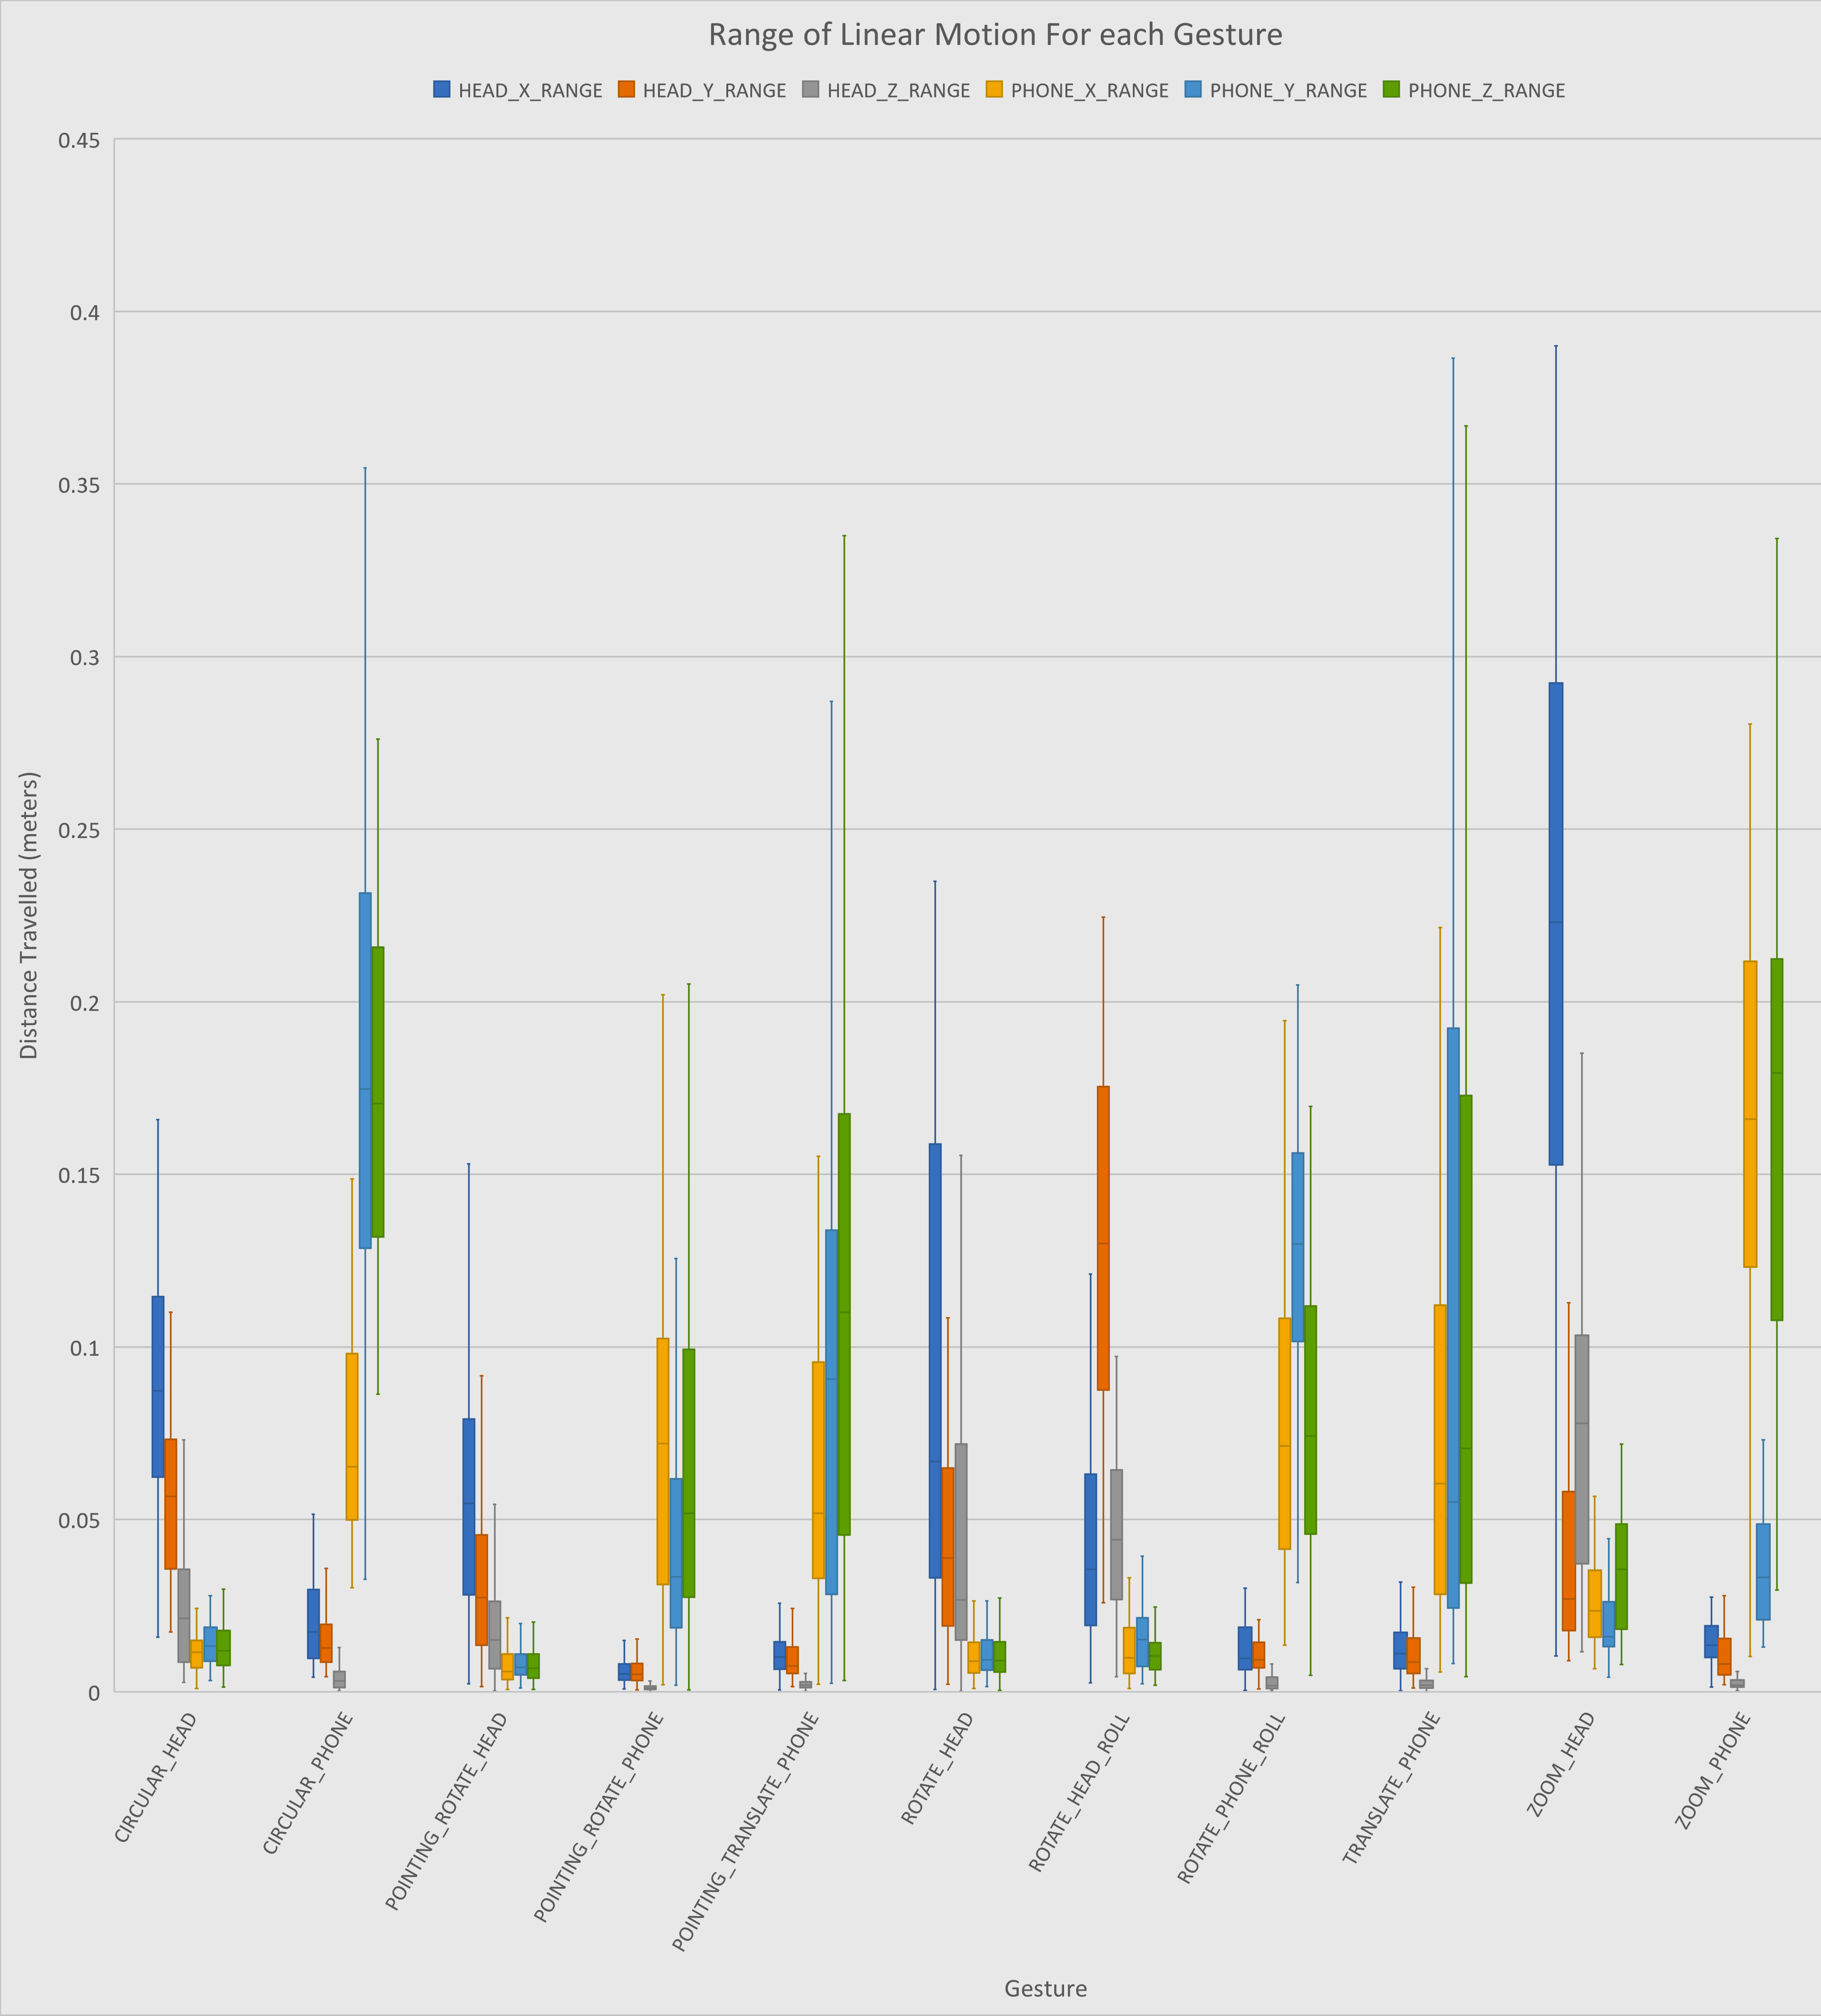
\includegraphics[width=0.9\textwidth]{figures/RangeOfLinearMotion.png}
    \caption{\label{fig:range_of_linear_motion} Range of linear motion for each gesture, in meters}
    \Description{Box and Wisker plot showing the mean, min, max, and the first and third quartiles for the observed range of linear motion for each gesture recorded.}
\end{figure*}
In total we were able to record 1028 gestures. The sample rate for the images was between 30-33 images per second, and the IMU sample rate was an expected 50$Hz$.
A breakdown of the range of linear motion can be seen in \autoref{fig:range_of_linear_motion}.
From this we can see the axis with the greatest movement typically correlate to the object being moved, e.g. the head or the phone, which is to be expected and helps to confirm the MoCap data is accurate.
The gesture with the most movement in any given axis was for moving the head towards and away from the phone, with movement typically being between 15-30cm. However the gestures that involved the most movement across multiple axis were the ones that involved the translation of the phone, which typically saw movement across all three axis.

Unfortunately we are unable to accurately breakdown the range of angular motion as we do not record the amount of rotation performed, only the exact rotation observed. As such we have some issues with rotations being calculated as around 360\textdegree / 2$\pi$. None of the gestures performed by the participants actually required a rotation that large, however due to the cyclical nature of angles, you can rotate a small amount and end up with a larger angle if you try to take the difference between frames. 
This only seems to have impacted the calculation for roll, calculated yaw and pitch appear correct. This is due to the orientation of the participant during recording ensuring that the observed pitch and yaw never exceeding 360\textdegree or falling below 0\textdegree. A breakdown of the angular motion with can be found under \autoref{app:study_data}, however the calculated roll is unfortunately incorrect.
Reviewing the data we do have however does show that the MoCap data is consistent with what we would expect, showing all accurate rotations never exceeding 180\textdegree, rotation being very small during linear motion gestures, and that head gestures typically require greater rotation than those of the phone.

By using a face detector~\cite{yu2022yunet} with OpenCV we were able to generate a breakdown of the percentage of images within which a face could be detected. The percentage of frames with a face detected for each gesture, and variant of a gesture, is available as an appendix under \autoref{app:study_data}, along with a breakdown of average time elapsed performing a gesture. 
From the table we can see that some gestures have much lower frequency of frames wherein the head is detected. Most of these are to be expected, such as the gestures that rotate the phone, which can cause the camera's point of view to no longer include the face. A particular example is the Bottom-Centre variant of the Pointing-Rotate-Phone gesture, which involves the phone being tilted such that the top of the phone is tilted away from the participant's face. Given the front-facing camera is mounted on the top, this will result in the camera moving the furthest from the face.

On average all the gestures took between 2.4 - 3.6 seconds, with the circular and zoom motions, for both head and phone, taking the longest to perform.

\subsection{Data Synchronisation and Post-Processing}
Before being able to use the data for training, we needed to synchronise the data recorded from the smartphone, and the fbx data from the MoCap studio.
To do this we derived the acceleration of the phone based on the MoCap data to find where it meets/exceeds the magnitude of the shake recorded by the app. From this we can determine the frame of the fbx data that corresponds to the recorded timestamp. We can determine the frame for any subsequent timestamp based on the known frame-rate of 60fps. 
To verify the data didn't drift we resync the data based on the other 2 recorded shakes, verifying that they're within 10 frames of the expected frame. In doing this verification, we did not come across any recording wherein subsequent shakes were not found to be at the expected frame.
The synchronisation was performed with a Python script that was run within Blender after loading in the fbx.
Blender was used as it permitted viewing the fbx data so that we could verify the frames the shake was detected by watching the playback. We could also use Blender to verify the derived location, roll, pitch, and yaw were correct by inserting a plane into the scene and assigning it the derived values, checking that it lined-up through all of the motion trackers.
The other reason for using Blender is that it allowed us to programmatically access the fbx file as a data structure and therefore write a script capable of deriving the required head and phone poses from the fbx, and then sync it with the data recorded from the phone.
Synchronised data was exported to CSVs for each motion recording, containing a path to the image, the raw IMU data, and the derived MoCap data.

An additional stage of pre-processing that was performed was to generate the RGB images from the YUV data captured by the phone. This was performed with a Python script and the OpenCV library.